% Sets page margins to 1", which is the academic standard
% allows the included extensions of graphic files
% sets graphic path, does not currently work because of space in folder name
% I do not remember what this does
% allows the xhead parameters (text on the top right/left areas of pages)
% \setcounter{tocdepth}{the number of depth}
% INCLUDEGRAPHICS EXPLANATION
% \newline \includegraphics[scale=1]{name of file}
% sometimes you want to twice encase the filename in squiggly brackets. I do not know why but sometimes it is required.


\documentclass{article}
%%%%%%%%%%%%%%%%%%%%%%%%%%%%%%%%%%%%%%%%%%%%%%%%%%%%%%%%%%%%%%%%%%%%%%%%%%%%%%%%%%%%%%%%%%%%%%%%%%%%%%%%%%%%%%%%%%%%%%%%%%%%%%%%%%%%%%%%%%%%%%%%%%%%%%%%%%%%%%%%%%%%%%%%%%%%%%%%%%%%%%%%%%%%%%%%%%%%%%%%%%%%%%%%%%%%%%%%%%%%%%%%%%%%%%%%%%%%%%%%%%%%%%%%%%%%
\usepackage{geometry}
\usepackage{fancyhdr}
\usepackage[pdftex]{graphicx}

%TCIDATA{OutputFilter=LATEX.DLL}
%TCIDATA{Version=5.50.0.2953}
%TCIDATA{<META NAME="SaveForMode" CONTENT="1">}
%TCIDATA{BibliographyScheme=Manual}
%TCIDATA{Created=Monday, January 30, 2012 17:20:46}
%TCIDATA{LastRevised=Tuesday, March 20, 2012 10:40:12}
%TCIDATA{<META NAME="GraphicsSave" CONTENT="32">}
%TCIDATA{<META NAME="DocumentShell" CONTENT="Standard LaTeX\Blank - Standard LaTeX Article">}
%TCIDATA{CSTFile=40 LaTeX article.cst}

\newtheorem{theorem}{Theorem}
\newtheorem{acknowledgement}[theorem]{Acknowledgement}
\newtheorem{algorithm}[theorem]{Algorithm}
\newtheorem{axiom}[theorem]{Axiom}
\newtheorem{case}[theorem]{Case}
\newtheorem{claim}[theorem]{Claim}
\newtheorem{conclusion}[theorem]{Conclusion}
\newtheorem{condition}[theorem]{Condition}
\newtheorem{conjecture}[theorem]{Conjecture}
\newtheorem{corollary}[theorem]{Corollary}
\newtheorem{criterion}[theorem]{Criterion}
\newtheorem{definition}[theorem]{Definition}
\newtheorem{example}[theorem]{Example}
\newtheorem{exercise}[theorem]{Exercise}
\newtheorem{lemma}[theorem]{Lemma}
\newtheorem{notation}[theorem]{Notation}
\newtheorem{problem}[theorem]{Problem, T2}
\newtheorem{proposition}[theorem]{Proposition}
\newtheorem{remark}[theorem]{Remark}
\newtheorem{solution}[theorem]{Solution}
\newtheorem{summary}[theorem]{Summary}
\newenvironment{proof}[1][Proof]{\noindent\textbf{#1.} }{\ \rule{0.5em}{0.5em}}
\geometry{left=1in,right=1in,top=1in,bottom=1in} 
\DeclareGraphicsExtensions{.pdf,.png,.jpg}
\graphicspath{{D:/Dropbox/Private/FP/Gruppe34/FellesDoc/D2BBT/Images/}}
\setlength{\headheight}{15.2pt}
\pagestyle{fancy}
\lhead{Group 34}
\rhead{FP: MMI D2}
\input{tcilatex}
\setcounter{secnumdepth}{-1}

\begin{document}


% begin title page, use \\ for newline
\begin{titlepage}
\title{Collaboration Project\\
\textbf{Evaluation of Paper Prototype}\\
Group 34}
% now one can list the authors, \textbf{} makes bold text
\author{Bj\o rn \AA ge Tungesvik\and Tina Syversen\and Andr\'e Philipp\and Odd Magnus Trondrud\and Eivind Kvissel\and H\aa vard H\o iby}
\maketitle
\end{titlepage}
\newpage

\part{The Design}

\section{Graphical User Interface}

Login dialogue\{0\}:\newline
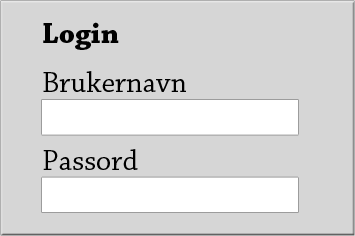
\includegraphics[scale=0.3]{Login.png}\newline
The calendar view\{1\}: \newline
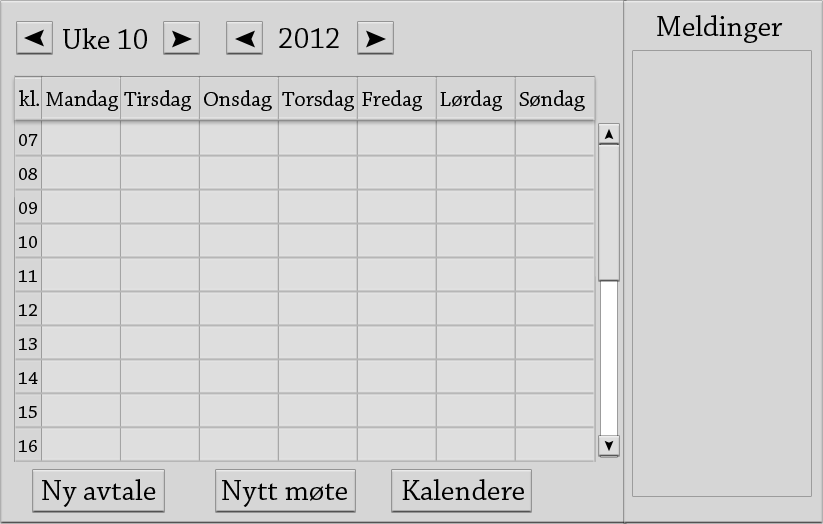
\includegraphics[scale=0.3]{Kalender.png}\newline
Calendar selection\{2\}: \newline
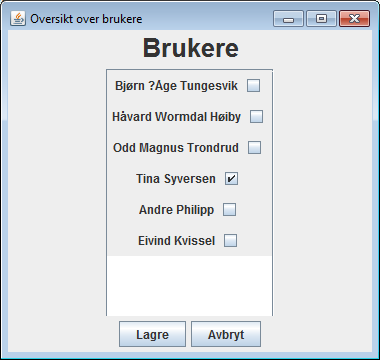
\includegraphics[scale=0.3]{kalendere.png}\newline
User selection\{3\}:\newline
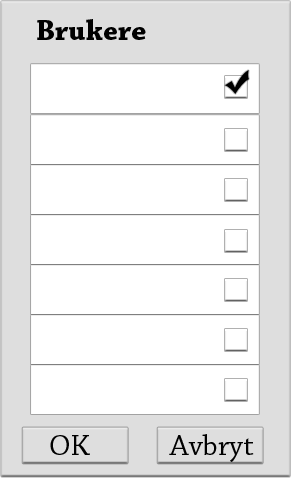
\includegraphics[scale=0.3]{brukere.png}\newline
Appointment edit-dialogue\{4\}: \newline
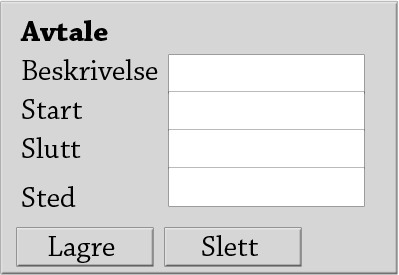
\includegraphics[scale=0.3]{Avtale.png}\newline
Datepick dialogue\{5\}: \newline
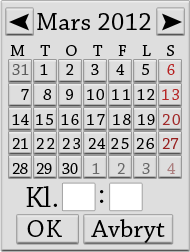
\includegraphics[scale=0.3]{datepicker.png}\newline
Meeting invitation dialogue\{6\}: \newline
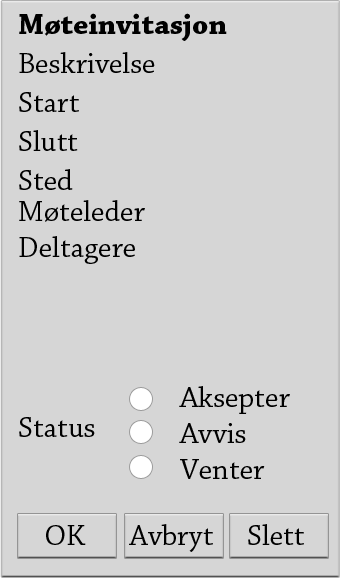
\includegraphics[scale=0.3]{moteinvite.png}\newline
Create-a-meeting dialogue\{7\}: \newline
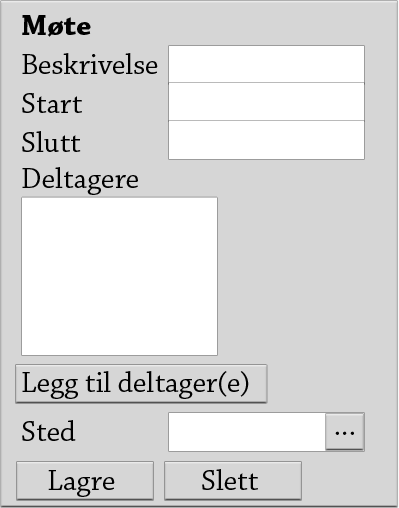
\includegraphics[scale=0.3]{mote.png}\newline
Meeting room booking dialogue\{8\}: \newline
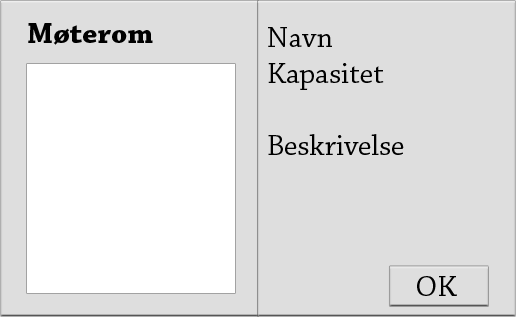
\includegraphics[scale=0.3]{moterom.png}

\section{State Diagram}

The picture illustrates the diagram while the following block of text
further explains what has to be pressed as I\ couldn't figure out how to get
text to appear above the arrows in the program.\newline
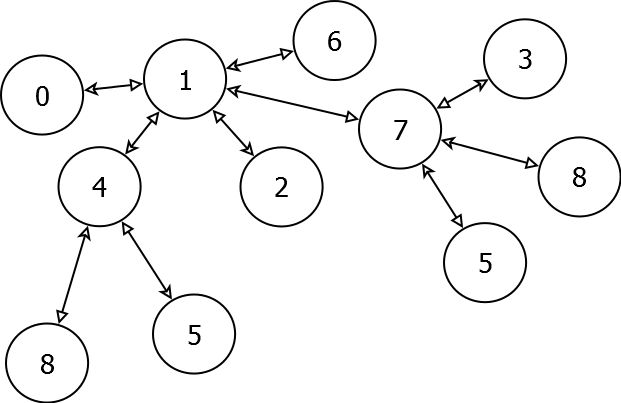
\includegraphics[scale=0.6]{tilstand.png}

Uppercase text describes a feature not visible in the design prototype.

FROM 0:

\qquad \TEXTsymbol{>}1:Login

FROM 1:

\qquad \TEXTsymbol{>}0:LOGOUT

\qquad \TEXTsymbol{>}2:"Kalendere"

\qquad \TEXTsymbol{>}4:"Ny avtale"

\qquad \TEXTsymbol{>}6:VIEW MEETING INVITE

\qquad \TEXTsymbol{>}7:"Nytt m\o te"

FROM 2:

\qquad \TEXTsymbol{>}1:OK/Avbryt

FROM\ 3:

\qquad \TEXTsymbol{>}7:"OK/Avbryt"

FROM 4:

\qquad \TEXTsymbol{>}1:"Lagre/Slett"

\qquad \TEXTsymbol{>}8:[...]

\qquad \TEXTsymbol{>}5:Start/Slutt

FROM 5:

\qquad \TEXTsymbol{>}4 ELLER \TEXTsymbol{>}7:"OK"

FROM 6:

\qquad \TEXTsymbol{>}1:"OK/Avbryt/Slett"

FROM 7:

\qquad \TEXTsymbol{>}3:"Legg til deltager(e)"

\qquad \TEXTsymbol{>}8:[...]

\qquad \TEXTsymbol{>}1:"Lagre/Slett"

\qquad \TEXTsymbol{>}5:Start/Slutt

FROM 8:

\qquad \TEXTsymbol{>}7/4:"OK"
\newpage
\part{Testing}

\section{Scenarios}

We chose to use the scenarios supplied to us through the DB-D2 description
document. Yes, the ones on the last page of the document.

\section{Tasks}

Regular text describes the tasks presented to the user. \textit{Italicized
text} describes events performed by the computer when the user reached the
corresponding point.

\begin{enumerate}
\item Create a new appointment at 13:00 on the next Friday and book a
meeting room with a capacity of at least four people for this appointment.

\item Create a new meeting at 12:00-14:00 on the upcoming Wednesday and
invite Beate, Morten and Finn to it.

\item \textit{Receive invitation to board meeting at 12:00-14:00 on the
upcoming Wednesday. }Move earlier created meeting to 14:00-16:00 on the same
day.

\item \textit{Receive notification about Morten having declined your meeting
invite. }Remove Morten from the 14:00-16:00 Wednesday meeting.

\item Cancel the 14:00 meeting with Beate and Finn.
\end{enumerate}

\section{Procedure}

The prototype was tested on three members members from group 32. The tests
were conducted by members of group 34.

\section{Results}

After completing the tests and discussing our different designs with group
32, some design-flaws and absent features were revealed to us.

\subsection{Issues}

An issue of type 1 ("T1") indicates an outright error in the design, due to
an oversight or what not.

Type 2 ("T2")\ indicates a problem related to our design choices, while Type
3 ("T3") indicates that a or several design choices were confusing.

\bigskip

\textbf{Problem, T3:} The system's automatic completion of a
meeting/appointment's "end time"\ was regarded as confusing.

\textbf{Reason:} Upon entering a start-datetime for a meeting/appointment,
the end-datetime is automatically set to one hour after the start-datetime.
The confusion might have arisen from the slow handling of this automatic
completion due to the test being performed with pieces of paper.

\textbf{Fix:} None. We have decided to retain this functionality.

\bigskip

\textbf{Problem, T3: }Should an error-message appear when attempting to save
a meeting/appointment without specifying a location?

\textbf{Answer:} According to the specifications, an appointment does not
require a location, although meetings do.

\textbf{Fix:} Disallow saving a meeting unless a location is specified.

\bigskip

\textbf{Problem, T3:} Should it be possible to have several meetings or
appointments at the same datetime?

\textbf{Answer:} Yes.

\textbf{Fix:} Implement it.

\bigskip

\textbf{Problem, T2: }The datetime-selection window felt confusing.

\textbf{Reason:} The testing was performed with pieces of paper with
incorrect scaling.

\textbf{Fix:} None. The usability should improve when the system is
digitalized.

\bigskip

\textbf{Problem, T1:} The room-reservation dialogue has no "cancel"\ button.

\textbf{Reason:} Oversight.

\textbf{Fix:} Add a "cancel"\ button.

\bigskip

\textbf{Problem, T2:} Confusion regarding at what time a day begins.

\textbf{Reason:} The scrollbar on the right side of the calendar is shown
being scrolled all the way up but the earliest time shown is 07:00.

\textbf{Fix:} yep

\bigskip

\textbf{Problem, T2:} The location-field in the create/edit
meeting/appointment dialogue window felt ambiguous.

\textbf{Reason:} The [...]-button in the location-field.

\textbf{Fix:} Seperate the location field and the [...]\ (book-a-room) and
remove any ambiguity as to whether one can use both.

\bigskip

\textbf{Problem, T1}: Calendar-view does not display the date.

\textbf{Reason:} Oversight.

\textbf{Fix:} Add the week's dates to the calendar-view.

\bigskip

\textbf{Problem, T1:} The book-a-room-dialogue window displays all the
meeting rooms in the system, not just the ones that are available at the
selected time.

\textbf{Reason:} Oversight.

\textbf{Fix:} It's simple, all we have to do is make the system not display
the rooms that are already reserved for the given time.

\bigskip

\textbf{Problem, T3:} Should the user be prompted to create a new
meeting/appointment by clicking on the calendar?

\textbf{Answer:} Possibly. Perhaps while holding down a modifier key while
left-clicking, or through the right-click dialogue?

\textbf{Fix:} Yes.

\bigskip

\textbf{Problem, T2:} A lot of windows.

\textbf{Reason:} Testers reported that the amount of dialogue-windows they
had to click through was startling.

\textbf{Fix:} We should investigate if some of the dialogue-windows can be
combined or solved in an alternative manner.

\subsection{Questionnaire Results}

After the test was completed, the tester was given the questionnaire found
at this subject's (DB) "\O vinger/\O ving D2a - Pilottesting" page on
itslearning.

Q\#\ is Question number \#.

A\# is how many testers that selected \# as their answer to the question.

\begin{tabular}{|l|l|l|l|l|l|}
\hline
& \textbf{A1} & \textbf{A2} & \textbf{A3} & \textbf{A4} & \textbf{A5} \\ 
\hline
\textbf{Q1} & $0$ & $0$ & $1$ & $2$ & $0$ \\ \hline
\textbf{Q2} & $1$ & $0$ & $2$ & $0$ & $0$ \\ \hline
\textbf{Q3} & $0$ & $0$ & $0$ & $2$ & $1$ \\ \hline
\textbf{Q4} & $2$ & $1$ & $0$ & $0$ & $0$ \\ \hline
\textbf{Q5} & $0$ & $0$ & $0$ & $1$ & $2$ \\ \hline
\textbf{Q6} & $1$ & $2$ & $0$ & $0$ & $0$ \\ \hline
\textbf{Q7} & $0$ & $0$ & $1$ & $0$ & $2$ \\ \hline
\textbf{Q8} & $2$ & $1$ & $0$ & $0$ & $0$ \\ \hline
\textbf{Q9} & $0$ & $0$ & $1$ & $0$ & $2$ \\ \hline
\textbf{Q10} & $1$ & $2$ & $0$ & $0$ & $0$ \\ \hline
\end{tabular}
\newpage

\part{The Revised Design}

Having completed the tests, the following screens have been visually
redesigned:

\bigskip 

MANGLER: kalender-view med dato p\aa\ ukedagene og fikset scrollbar

Create-a-meeting dialogue: \newline
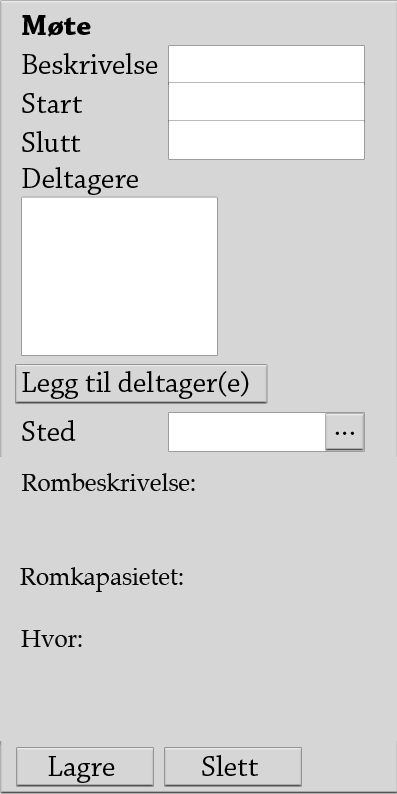
\includegraphics[scale=0.3]{mote2.png}\newline

\end{document}
